\documentclass{article}
\usepackage[utf8]{inputenc}
\usepackage[margin=1in]{geometry}
\usepackage{amsmath, amsfonts}
\usepackage{fancyhdr}
\usepackage{multicol}
\usepackage{graphicx}
\graphicspath{ {images/} }
\pagestyle{empty}
\fancyhf{}
\cfoot{\thepage}

\lhead{MATB42: Assignment \#2 \\
Bonus}
\rhead{
Poon, Keegan\\
1002423727\\
Jan 30th 2018}

\renewcommand{\headrulewidth}{0pt}
\begin{document}

\thispagestyle{fancy}

\begin{enumerate}
\item Let $\displaystyle f(x) = 
\begin{cases}
        0, &- \pi < x < -\frac{\pi}{2} \\
        2, &- \frac{\pi}{2}\leq x < \frac{\pi}{2} \\
        0, & \frac{\pi}{2} \leq x < \pi
\end{cases}
$
\begin{enumerate}
\item Find the Fourier series of $f$.
\begin{multicols}{2}
\noindent

\begin{align*}
a_0 &= \frac{1}{\pi} \int_{-\pi}^{\pi}f(x)dx \\
&= \frac{1}{\pi} \Bigg[ \int_{-\pi}^{-\frac{\pi}{2}}0dx + \int_{-\frac{\pi}{2}}^{\frac{\pi}{2}}2dx + \int_{\frac{\pi}{2}}^{\pi}0dx \Bigg]\\
&= \frac{1}{\pi} \Bigg[2\pi\Bigg]\\
&= 2
\end{align*}

\begin{align*}
b_k &= \frac{1}{\pi} \int_{-\pi}^{\pi}f(x)\sin(kx)dx \\
&= \frac{2}{\pi} \int_{-\frac{\pi}{2}}^{\frac{\pi}{2}}\sin(kx)dx \\
&= 0 \: \: \: [\text{sin is odd}]
\end{align*}

\begin{align*}
a_k &= \frac{1}{\pi} \int_{-\pi}^{\pi}f(x)\cos(kx)dx \\
&= \frac{2}{\pi} \int_{-\frac{\pi}{2}}^{\frac{\pi}{2}}\cos(kx)dx \\
&= \frac{2}{k\pi} \Bigg[\sin(kx)\Bigg]_{-\frac{\pi}{2}}^{\frac{\pi}{2}} \\
&= \frac{2}{k\pi} \Bigg[2\sin\Big(\frac{k\pi}{2}\Big)\Bigg]\\
&= \frac{4}{k\pi} \sin\Big(\frac{k\pi}{2}\Big)
\end{align*}
This is 0 for even elements, and alternating between 1 and -1 for odd elements.
\end{multicols}

Therefore the Fourier polynomial (for the non-zero terms) is 
\[
    1 + \sum_{l=1}^{\infty} \Bigg[ \frac{4(-1)^{l+1}}{(2l-1)\pi}\cos((2l-1)x)\Bigg]
\]
\item Determine if the Fourier series in part (a) converges. If it does converge, what are the values to which it converges (on $[-\pi, \pi]$).

The function is continuous on its partitions (they are constant functions), so by the theorem the polynomial converges to $f(x)$ on the continuous intervals. On the discontinuities, it converges to 0 at $\frac{\pi}{2}$ and $\frac{-\pi}{2}$ from the Fundemental theorem, and to 0 at $\pi$ and $-\pi$.
\item Use symbolic algeba software to sketch $f(x)$ and its $4^{th}$ degree Fourier polynomial over the interval $[-3\pi,3\pi]$.

        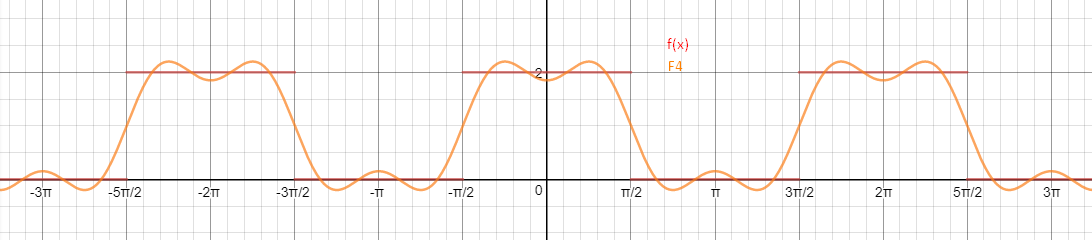
\includegraphics[width=\textwidth]{b42-a2-2c}
\end{enumerate}
\newpage
\item \begin{enumerate}
\item Find the Fourier series of the function $f(x)$ defined by $\displaystyle f(x) = \begin{cases}
0 &,-\pi \leq x < 0 \\
x &, 0\leq x < \pi
\end{cases}
$ and extended from this with period $2\pi$ to all of $\mathbb{R}$.

If this Fourier series converges describe the function to which it converges.
        \begin{multicols}{2}
        \noindent
        \begin{align*}
            a_0 &= \frac{1}{\pi} \int_{-\pi}^{\pi}f(x) dx \\
            &= \frac{1}{\pi} \Bigg[\int_{-\pi}^{0}f(x) dx + \int_{0}^{\pi}f(x) dx \Bigg] \\
            &= \frac{1}{\pi} \Bigg[ 0 + \int_{0}^{\pi}x dx \Bigg] \\
            &= \frac{1}{\pi} \Bigg[\frac{1}{2}\Big[x^2\Big]_{0}^{\pi} \Bigg] \\
            &= \frac{\pi}{2}
        \end{align*}
        \begin{align*}
            a_k &= \frac{1}{\pi} \int_{-\pi}^{\pi}f(x)\cos(kx) dx \\
            &= \frac{1}{\pi} \Bigg[\int_{-\pi}^{0}0 dx + \int_{0}^{\pi}x\cos(kx) dx\Bigg] \\
            &\text{Let } u = x,\: du = dx,  \\
            & \: \: \:dv = \cos(kx),\: v = \frac{\sin(kx)}{k} \\
            &= \frac{1}{\pi} \Bigg[\frac{1}{k}\Big[x\sin(kx)\Big]^{\pi}_{0} - \frac{1}{k}\int_{0}^{\pi}\sin(kx) dx\Bigg] \\
            &= - \frac{1}{k\pi} \Bigg[\int_{0}^{\pi}\sin(kx) dx\Bigg] \\
            &= \frac{1}{k^2\pi} \Big[\cos(kx) \Big]_{0}^{\pi}\\
            &= \frac{(-1)^{-k} - 1}{k^2\pi} \\
        \end{align*}
        \begin{align*}
            b_k &= \frac{1}{\pi} \int_{-\pi}^{\pi}f(x)\sin(kx) dx \\
            &= \frac{1}{\pi} \Bigg[\int_{-\pi}^{0}0 dx +  \int_{0}^{\pi}x\sin(kx) dx \Bigg]\\
            &\text{Let } u = x,\: du = dx,\: dv = \sin(kx),\: v = -\frac{1}{k}\cos(kx) \\
            &= \frac{1}{\pi} \Bigg[-\frac{1}{k}\Big[x\cos(kx)\Big]^{\pi}_{0} + \frac{1}{k}\int_{0}^{\pi}\cos(kx) dx \Bigg]\\
            &= \frac{1}{k \pi} \Bigg[-\pi\cos(k\pi) + \frac{1}{k} \Big[ \sin(kx) \Big]_{0}^{\pi} \Bigg]\\
            &= \frac{1}{k \pi} \Bigg[-\pi\cos(k\pi) + 0 \Bigg]\\
            &= \frac{(-1)^{k+1}}{k}
        \end{align*}
        Therefore the Fourier series of $f$ is 
        \[
        F(x) = \frac{\pi}{4} + \sum^{\infty}_{k=1}\Bigg[ \frac{(-1)^k-1}{k^2\pi}\cos(kx) + \frac{(-1)^{k+1}}{k} \sin(kx) \Bigg]
        \]
        \end{multicols}
        Since $f$ is piecewise very smooth (0, $x$ are infinitely differentiable), the series converges to $f$ on $(-\pi,\pi)$ and on both endpoints, it converges to $\frac{\pi}{2}$.
        
\item Using the series from part (a) show that 
\[
\frac{\pi^2}{8} = 1 + \frac{1}{3^2} + \frac{1}{5^2} + \frac{1}{7^2} + \cdots .
\]

\begin{multicols}{2}
\noindent
\begin{align*}
        F(0) &= \frac{\pi}{4} + \sum^{\infty}_{k=1}\Bigg[ \frac{(-1)^k-1}{k^2\pi} \Bigg] \\ 
        0 &= \frac{\pi}{4} + \sum^{\infty}_{k=1}\Bigg[ \frac{-2}{(2k - 1)^2\pi} \Bigg] \\
        \end{align*}
        \begin{align*}
         \frac{\pi}{4} &= \sum^{\infty}_{k=1}\Bigg[ \frac{2}{(2k - 1)^2\pi} \Bigg] \\
         \frac{\pi^2}{8} &= \sum^{\infty}_{k=1} \frac{1}{(2k - 1)^2} \\
\end{align*}
\end{multicols}
\end{enumerate}
\newpage
\item Find the Fourier series for the restriction of the function $f(x) = 3 + 3x$ to each of the following intervals, $[a,b]$. If the Fourier series converges, to what values will the series converge at the end points?
\begin{enumerate}
\item $[a,b] = [-\pi, \pi] $
\begin{multicols}{2}
\noindent
\begin{align*}
    a_0 &= \frac{1}{\pi} \int_{-\pi}^{\pi}f(x) dx \\
    &= \frac{1}{\pi} \int_{-\pi}^{\pi}3 + 3x dx \\
    &= \frac{1}{\pi} \Bigg[6\pi +  \frac{3}{2}\Big[x^2\Big]^{\pi}_{-\pi}\Bigg] \\
    &= \frac{1}{\pi} \Bigg[6\pi + 0 \Bigg] \\
    &= 6\\
\end{align*}
\begin{align*}
    a_k &= \frac{1}{\pi} \int_{-\pi}^{\pi}f(x)\cos(kx) dx \\
    &= \frac{3}{\pi}\Bigg[ \int_{-\pi}^{\pi}\cos(kx) dx + \int_{-\pi}^{\pi}x\cos(kx) dx \Bigg] \\
    &= \frac{6}{k\pi}\Big[\sin(kx)\Big]_{0}^{\pi} \: \: \: [\text{Since $x$ odd and cos even}] \\
    &= 0
\end{align*}
\begin{align*}
    b_k &= \frac{1}{\pi} \int_{-\pi}^{\pi}f(x)\sin(kx) dx \\
    &= \frac{3}{\pi}\Bigg[ \int_{-\pi}^{\pi}\sin(kx) dx + \int_{-\pi}^{\pi}x\sin(kx) dx \Bigg] \\
    &= \frac{6}{\pi}\Bigg[ \int_{0}^{\pi}x\sin(kx) dx \Bigg] \: \: \: [\text{Since $x$ and sin odd}] \\
    &\text{Let $u = x, du = 1 dx, dv = \sin(kx) dx, v = -\frac{\cos(kx)}{k}$} \\
    &= \frac{6}{\pi}\Bigg[ -\frac{1}{k}\Big[x\cos(kx)\Big]^{\pi}_{0} + \frac{1}{k}\int^{\pi}_{0}\cos(kx)dx \Bigg] \\
    &= \frac{6}{k\pi}\Bigg[ \pi(-1)^{k+1} +  \frac{1}{k}\Big[\sin(kx)\Big]^{\pi}_{0} \Bigg] \\
    &= \frac{6(-1)^{k+1}}{k}\\ 
    \end{align*} 
    Therefore the Fourier series is defined as 
    \[
        F(x) = 3 + \sum_{k=1}^{\infty}\frac{6(-1)^{k+1}}{k}\sin(kx)
    \]
    Linear functions are infinitely differentiable so it will converge to $f(x)$ within the interval, and coverges to 3 at the endpoints.
    \end{multicols}
    \newpage
\item $[a,b] = [0, 2\pi]$

\begin{multicols}{2}
\noindent
\begin{align*}
    a_0 &= \frac{1}{\pi} \int_{-\pi}^{\pi}f(x) dx \\
    &= \frac{1}{\pi} \int_{0}^{2\pi}3 + 3x dx \\
    &= \frac{1}{\pi} \Bigg[6\pi +  \frac{3}{2}\Big[x^2\Big]^{2\pi}_{0}\Bigg] \\
    &= \frac{1}{\pi} \Bigg[6\pi + 6\pi^2 \Bigg] \\
    &= 6(\pi + 1)\\
\end{align*}
\begin{align*}
    a_k &= \frac{1}{\pi} \int_{-\pi}^{\pi}f(x)\cos(kx) dx \\
    &= \frac{3}{\pi}\Bigg[ \int_{0}^{2\pi}\cos(kx) dx + \int_{0}^{2\pi}x\cos(kx) dx \Bigg] \\
    &\text{Let } u = x,\: du = dx,\: dv = \cos(kx),\: v = \frac{1}{k}\sin(kx) \\
    &= \frac{3}{k\pi}\Bigg[\Big[\sin(kx)\Big]_{0}^{2\pi} + \Big[x \sin(kx)\Big]^{2\pi}_{0} - \int_{0}^{2\pi} \sin(kx) dx\Bigg] \\
    &= -\frac{3}{k^2\pi}\Big[\cos(kx)\Big]_{0}^{2\pi} \\
    &= 0 \\
\end{align*}
\begin{align*}
    b_k &= \frac{1}{\pi} \int_{-\pi}^{\pi}f(x)\sin(kx) dx \\
    &= \frac{3}{\pi}\Bigg[ \int_{0}^{2\pi}\sin(kx) dx + \int_{0}^{2\pi}x\sin(kx) dx \Bigg] \\
    &\text{Let $u = x, du = 1 dx, dv = \sin(kx) dx, v = -\frac{\cos(kx)}{k}$} \\
    &= \frac{3}{k\pi}\Bigg[ \Big[\cos(kx)\Big]_{0}^{2\pi} - \Big[x\cos(kx)\Big]_{0}^{2\pi} + \int_{0}^{2\pi}\cos(kx) dx \Bigg] \\
    &= \frac{3}{k\pi}\Bigg[ -2\pi + \frac{1}{k} \Big[\sin(kx)\Big]_{0}^{2\pi}  \Bigg] \\
    &= -\frac{6}{k}\\ 
    \end{align*} 
    \end{multicols}
    Therefore the Fourier series is defined as 
    \[
        F(x) = 3(\pi + 1) - \sum_{k=1}^{\infty}\frac{6}{k}\sin(kx)
    \]
    Linear functions are infinitely differentiable so it will converge to $f(x)$ within the interval, and coverges to $3+3\pi$ at the endpoints.
\end{enumerate}

\newpage

\item Find the Fourier series of the function $f(x)$ defined on $[0,2\pi]$ by $f(x) = x(x-2\pi)$ and extended from this with period $2\pi$ to all of $\mathbb{R}$. Use symbolic algebra software to graph the $4^{th}$ degree Fourier polynomial together with the original function.
\begin{multicols}{2} 
\noindent

\begin{align*}
    b_k &= \frac{1}{\pi} \int_{-\pi}^{\pi}f(x)\sin(kx) dx \\
    &= \frac{1}{\pi} \int_{0}^{2\pi} x(x-2\pi) dx \\
    &= \frac{1}{\pi} \Bigg[ \int_{0}^{2\pi} x^2\sin(kx) dx - 2\pi\int_{0}^{2\pi} x\sin(kx) dx \Bigg] \\
    &\text{Let } u = x,\: du = dx,\: dv = \sin(kx),\: v = -\frac{1}{k}\cos(kx) \\
    &= \frac{1}{\pi} \Bigg[ \int_{0}^{2\pi} x^2\sin(kx) dx - 2\pi\Big( -\frac{1}{k} \Big[ x\cos(kx)\Big]_{0}^{2\pi} \\
    & \: \: \: + \frac{1}{k}\int_{0}^{2\pi} \cos(kx) dx \Big) \Bigg] \\
    &= \frac{1}{\pi} \Bigg[ \int_{0}^{2\pi} x^2\sin(kx) dx - 2\pi\Big( -\frac{2\pi}{k} \\ 
    & \: \: \: + \frac{1}{k^2} \Big[\sin(kx) \Big]_{0}^{2\pi} \Big) \Bigg] \\
    &= \frac{1}{\pi} \Bigg[ \int_{0}^{2\pi} x^2\sin(kx) dx + \frac{4\pi^2}{k} \Bigg] \\
    &\text{Let }u = x^2, du = 2xdx, \\
    & \: \: \: dv = \sin(kx) dx, v = -\frac{\cos(kx)}{k} \\
    &= \frac{1}{k\pi} \Bigg[ -\Big[ x^2 \cos(kx) \Big]_{0}^{2\pi} + \int_{0}^{2\pi} x\cos(kx) dx  + 4\pi^2 \Bigg] \\
    &\text{Let } u = x,\: du = dx,\: dv = \sin(kx),\: v = -\frac{1}{k}\cos(kx) \\
    &= \frac{1}{k\pi} \Bigg[  \frac{1}{k}\Big[ x\sin(kx) \Big]_{0}^{2\pi} - \frac{1}{k}\int_{0}^{2\pi} \cos(kx) dx \Bigg] \\
    &= \frac{1}{k\pi} \Bigg[  - \frac{1}{k^2}\Big[ \sin(kx) \Big]_{0}^{2\pi} \Bigg] \\
    &= 0
\end{align*} 

\begin{align*}
    a_k &= \frac{1}{\pi} \int_{-\pi}^{\pi}f(x)\cos(kx) dx \\
    &= \frac{1}{\pi} \Bigg[\int_{0}^{2\pi} x^2\cos(kx) dx - 2\pi \int_{0}^{2\pi} x \cos(kx) dx \Bigg]\\
    &\text{Let $u = x^2, du = 2xdx, dv = \cos(kx) dx, v = \frac{\sin(kx)}{k}$} \\
    &= \frac{1}{\pi} \Bigg[\frac{1}{k}\Big[x^2\sin(kx)\Big]_{0}^{2\pi}  - \frac{2}{k}\int_{0}^{2\pi}x\sin(kx)dx  \\
    & \: \: \: - 2\pi\int_{0}^{2\pi} x \cos(kx) dx \Bigg]\\
    &= \frac{1}{\pi} \Bigg[- \frac{2}{k}\int_{0}^{2\pi}x\sin(kx)dx - 2\pi\int_{0}^{2\pi} x \cos(kx) dx \Bigg]\\
    &\text{Let $u = x, du = dx, dv = \sin(kx) dx, v = -\frac{\cos(kx)}{k}$} \\
    &= \frac{1}{\pi} \Bigg[ \frac{2}{k^2}\Big[x\cos(kx) \Big]_{0}^{2\pi} - \frac{1}{k}\int_{0}^{2\pi}\cos(kx)dx \\
    & \: \: \: - 2\pi\int_{0}^{2\pi} x \cos(kx) dx \Bigg]\\
    &= \frac{1}{\pi} \Bigg[ \frac{4\pi}{k^2} - \frac{1}{k^2} \Big[ \sin(kx) \Big]_{0}^{2\pi} - 2\pi\int_{0}^{2\pi} x \cos(kx) dx \Bigg]\\
    &\text{Let } u = x,\: du = dx,\: dv = \cos(kx),\: v = \frac{1}{k}\sin(kx) \\
    &= \frac{1}{\pi} \Bigg[ \frac{4\pi}{k^2} - 2\pi\Big(\frac{1}{k}\Big[ x\sin(kx)\Big]_{0}^{2\pi} - \frac{1}{k}\int_{0}^{2\pi}\sin(kx)dx \Big)\Bigg]\\
    &= \frac{1}{\pi} \Bigg[ \frac{4\pi}{k^2} + \frac{2\pi}{k}\int_{0}^{2\pi}\sin(kx)dx \Bigg]\\
    &= \frac{1}{\pi} \Bigg[ \frac{4\pi}{k^2} + \frac{2\pi}{k^2}\Big[ \cos(kx)\Big]_{0}^{2\pi}\Bigg]\\
    &= \frac{4}{k^2}
\end{align*} 
\end{multicols}
\begin{align*}
    a_0 &= \frac{1}{\pi} \int_{-\pi}^{\pi}f(x) dx \\
    &= \frac{1}{\pi} \int_{0}^{2\pi}x(x-2\pi)dx \\
    &= \frac{1}{\pi} \Bigg[ \int_{0}^{2\pi}x^2dx -\int_{0}^{2\pi}2x\pi dx \Bigg]\\
    &= \frac{1}{\pi} \Bigg[ \frac{1}{3}\Big[x^3\Big]_{0}^{2\pi} - \pi\Big[x^2 \Big]_{0}^{2\pi}\Bigg]\\
    &= \frac{1}{\pi} \Bigg[ \frac{8\pi^3}{3} - 4\pi^3 \Bigg]\\
    &= -\frac{4\pi^2}{3} \\
\end{align*} 
Therefore the Fourier series of $f$ is 
\[F(x) = -\frac{2\pi^2}{3} + \sum_{k=1}^{\infty} \frac{4}{k^2}\cos(kx) \]


        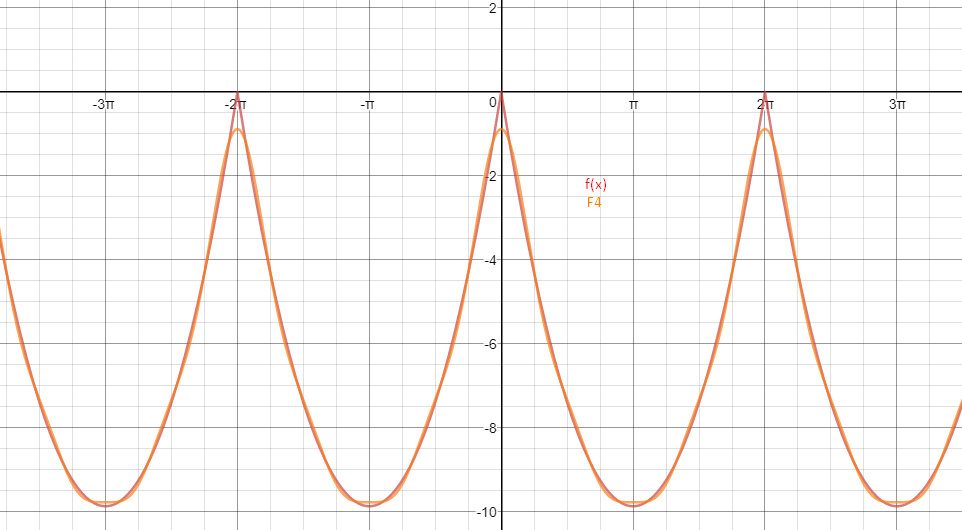
\includegraphics[width=\textwidth]{b42-a2-5a}
\newpage
\item Let $f(x)$ be defined on $[0,2\pi]$ by $f(x) = x(x-2\pi)$.
\begin{enumerate}
\item Find the Fourier cosine series of $f$.

From question 4, we can see that the function is already even, hence the Fourier series of the function itself is a cosine series of $f$. Namely 
\[ F(x) = -\frac{2\pi^2}{3} + \sum_{k=1}^{\infty} \frac{4}{k^2}\cos(kx) \]

\item Find the Fourier sine series of $f$.

To extend this as an odd function, define the $f$ on the range $[-2\pi,0]$ as $f(x) = -((x + 2\pi)((x + 2\pi)-2\pi)) = -x(x + 2\pi)$. Note that this definition of $f$ now has a period of $4\pi$.

\begin{align*}
    b_k &= \frac{1}{2\pi} \int_{-2\pi}^{2\pi}f(x)\sin\Big(\frac{kx}{2}\Big) dx \\
    &=- \frac{1}{\pi} \Bigg[ \int_{-2\pi}^{0}x(x+2\pi)\sin\Big(\frac{kx}{2}\Big) dx \Bigg] \: \: \:  [\text{$f$ and sin are both odd so the integrand is even}]\\
    &=- \frac{1}{\pi} \Bigg[ \int_{-2\pi}^{0}x^2\sin\Big(\frac{kx}{2}\Big) dx + 2\pi \int_{-2\pi}^{0}x\sin\Big(\frac{kx}{2}\Big) dx \Bigg] \\
    &\text{Let }u = x^2, \: du = 2xdx, \: dv = \sin\Big(\frac{kx}{2}\Big) dx,\: v = -\frac{2\cos(\frac{kx}{2})}{k} \\
    &=- \frac{1}{\pi} \Bigg[ -\frac{2}{k}\Big[x^2\cos\Big(\frac{kx}{2}\Big) \Big]_{-2\pi}^{0} + \frac{4}{k}\int_{-2\pi}^{0}x\cos\Big(\frac{kx}{2}\Big)dx + 2\pi \int_{-2\pi}^{0}x\sin\Big(\frac{kx}{2}\Big) dx \Bigg] \\
    &=- \frac{1}{\pi} \Bigg[ \frac{8\pi^2(-1)^k}{k} + \frac{4}{k}\int_{-2\pi}^{0}x\cos\Big(\frac{kx}{2}\Big)dx + 2\pi \int_{-2\pi}^{0}x\sin\Big(\frac{kx}{2}\Big) dx \Bigg] \\
    &\text{Let } u = x,\: du = dx,\: dv = \cos\Big(\frac{kx}{2}\Big),\: v = \frac{2}{k}\sin\Big(\frac{kx}{2}\Big) \\
    &=- \frac{1}{\pi} \Bigg[ \frac{8\pi^2}{k}(-1)^k + \frac{4}{k^2}\Big[x\sin\Big(\frac{kx}{2}\Big) \Big]_{-2\pi}^{0} - \frac{8}{k^2}\int_{-2\pi}^{0}\sin\Big(\frac{kx}{2}\Big) dx + 2\pi \int_{-2\pi}^{0}x\sin\Big(\frac{kx}{2}\Big) dx \Bigg] \\
    &=- \frac{1}{\pi} \Bigg[ \frac{8\pi^2}{k}(-1)^k + \frac{16}{k^3}\Big[ \cos\Big(\frac{kx}{2}\Big) \Big]_{-2\pi}^{0} + 2\pi \int_{-2\pi}^{0}x\sin\Big(\frac{kx}{2}\Big) dx \Bigg] \\
    &\text{Let $u = x, du = dx, dv = \sin\Big(\frac{kx}{2}\Big) dx, v = -\frac{2\cos(\frac{kx}{2})}{k}$} \\
    &=- \frac{1}{\pi} \Bigg[ \frac{8\pi^2}{k}(-1)^k + \frac{16}{k^3}(1 - (-1)^k) + \frac{4\pi}{k} \Big( -\Big[x\cos\Big(\frac{kx}{2}\Big)\Big]_{-2\pi}^{0} + \int_{-2\pi}^{0}\cos\Big(\frac{kx}{2}\Big) dx \Big) \Bigg] \\
    &=- \frac{1}{\pi} \Bigg[ \frac{8\pi^2}{k}(-1)^k + \frac{16}{k^3}(1 - (-1)^k) + \frac{4\pi}{k} \Big(  2\pi(-1)^{k+1} + \frac{2}{k}\Big[\sin\Big(\frac{kx}{2}\Big)\Big]_{-2\pi}^{0} \Big) \Bigg] \\
    &=- \frac{1}{\pi} \Bigg[ \frac{8\pi^2}{k}(-1)^k + \frac{16}{k^3}(1 - (-1)^k) + \frac{8\pi^2}{k}(-1)^{k+1} \Bigg] \\
    &= \frac{16}{k^3\pi}((-1)^k - 1)
\end{align*} 
\begin{multicols}{2} 
\noindent
\begin{align*}
    a_0 &= \frac{1}{2\pi} \int_{-2\pi}^{2\pi}f(x) dx \\
    &= 0 \: \: \: [\text{Since $f$ is defined odd}]
\end{align*} 
\begin{align*}
    a_k &= \frac{1}{2\pi} \int_{-2\pi}^{2\pi}f(x)\cos\Big(\frac{kx}{2}\Big) dx \\
    &= 0 \: \: \: [\text{Since $f$ is defined odd}]
\end{align*} 
\end{multicols}

The Fourier sine series is thusly 
        \[ F(x) = \sum_{k=1}^{\infty} \frac{16}{k^3\pi}((-1)^k-1)\sin\Big(\frac{kx}{2}\Big) \]
\item Use symbolic algebra software to graph the $4^{th}$ degree Fourier polynomials from parts (a) and (b) together with the original function.

    Fourier cosine series:

        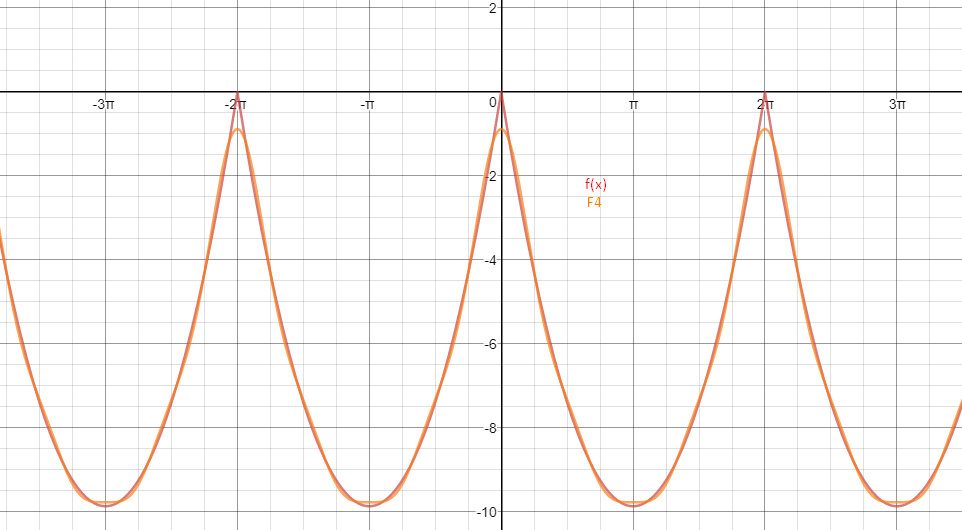
\includegraphics[width=\textwidth]{b42-a2-5a}

    Fourier sine series:

        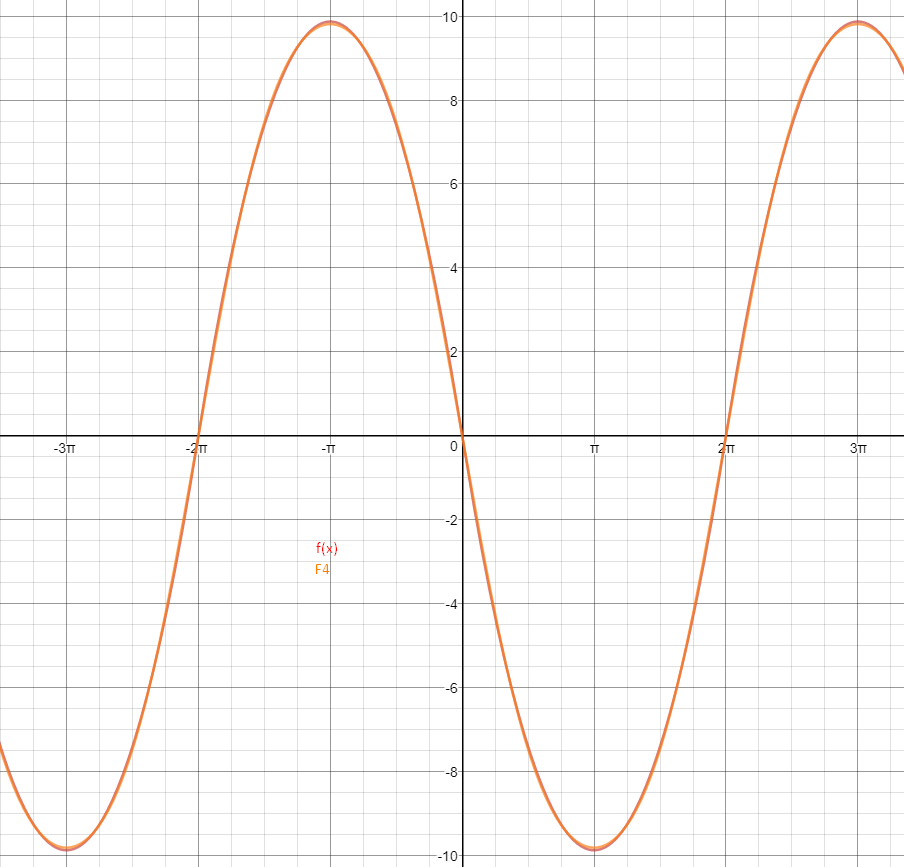
\includegraphics[width=10cm]{b42-a2-5b}
\end{enumerate}
\newpage
\item Find the Fourier series for the following functions:
\begin{enumerate}
\item $f(x) = \sin^2x + \sin^3x$
\begin{align*} 
\sin^2x + \sin^3x &= (1/2i)^2(e^{ix}-e^{-ix})^2 + (1/2i)^3(e^{ix}-e^{-ix})^3 \\
[\text{Binomial Theorem}]&= (-1/4)(e^{2ix} -2(e^{(ix-ix)}) + e^{-2ix}) + (-1/8i)(e^{3ix} -3(e^{(2ix-ix)}) +3(e^{(ix-2ix)}) - e^{-3ix}) \\
&=(-1/4)(e^{2ix} + e^{-2ix} -2) + (-1/8i)(e^{3ix} - e^{-3ix} -3(e^{(ix)}) +3(e^{(-ix)})) \\
&=(-1/2)(\cos(2x) -2) + (-1/4)(\sin(3x) -3\sin(x)) \\
&= 1 + \frac{3}{4}\sin(x) - \frac{1}{2}\cos(2x) - \frac{1}{4}\sin(3x)
\end{align*}
\item $f(x) = \sin^4x$
\begin{align*}
    \sin^4{x} &= (1/2i)^4(e^{ix} - e^{-ix})^4 \\
    [\text{Binomial Theorem}]&= (1/16)(e^{4ix} - 4e^{3ix-ix} + 6e^{2ix-2ix} - 4e^{ix-3ix} +e^{4ix}) \\
    &= (1/16)(6 - 4e^{2ix} - 4e^{-2ix}+ e^{4ix}  +e^{4ix}) \\
    &= (1/8)(3 - 4\cos(2x) + \cos(4x)) \\
    &= \frac{3}{8} - \frac{1}{2}\cos(2x) + \frac{1}{8}\cos(4x) \\
\end{align*}
\item $f(x) = \cos^7x$
\begin{align*}
\cos^7x &= (1/2)^7(e^{ix} + e^{-ix})^7 \\
[\text{Binomial Theorem}]&= (1/128)(e^{7ix} + 7e^{6ix-ix} + 21e^{5ix-2ix}+35e^{4ix-3ix} \\
& \: \: \: + 35e^{3ix-4ix} + 21e^{2ix-5ix} + 7e^{ix-6ix} + e^{-7ix} )\\
&= (1/128)(35e^{ix} + 35e^{-ix} + 21e^{3ix}+21e^{-3ix} +7e^{5ix} + 7e^{-5ix}+ e^{7ix} + e^{-7ix} )\\
&= (1/64)(35\cos(x) + 21\cos(3x) + 7\cos(5x) + \cos(7x))\\
&= \frac{35}{64}\cos(x) + \frac{21}{64}\cos(3x) + \frac{7}{64}\cos(5x) + \frac{1}{64}\cos(7x))\\
\end{align*}
( \textit{Hint:} Recall that $\cos \theta = \frac{e^{i\theta} + e^{-i\theta}}{2}$ and $\sin \theta = \frac{e^{i\theta} - e^{-i\theta}}{2i}$)
\end{enumerate}

The next question is for those among you who have previously seen complex numbers. It gives another approach to Fourier series.

\item Suppose
\begin{enumerate}
\item[] {}

\begin{enumerate}
\item $f(x)$ is a real values function of $x$,
\item $\displaystyle f(x) = \sum_{n=-\infty}^\infty C_ne^{inx}$ on $[-\pi, \pi ]$, where the $C_n$ are complex constants, and
\item that the term by term theorem holds true in this case
\end{enumerate}


\item Express the $C_n$ as integrals involving $f$.

Multiplying by $e^{-ikx}$ on both sides (where $k \in \mathbb{Z}$) gives the expression:
\begin{align*}
 e^{-ikx}f(x) &= \sum_{n=-\infty}^\infty C_ne^{inx}e^{-ikx} \\
 \implies \int_{-\pi}^{\pi}e^{-ikx}f(x) dx &= \int_{-\pi}^{\pi}\sum_{n=-\infty}^\infty C_ne^{inx - ikx}dx \\
 \int_{-\pi}^{\pi}e^{-ikx}f(x) dx &=  \sum_{n=-\infty}^\infty \int_{-\pi}^{\pi}C_ne^{i(n-k)x}dx \: \: \: [\text{Due to the term by term theorem}] \\
\end{align*}
Now there are two cases to consider as $n \in (-\infty, \infty)$
\begin{multicols}{2}
\noindent
When $n \not = k$
\begin{align*}
    \int_{-\pi}^{\pi}C_ne^{i(n-k)x}dx &= C_n\int_{-\pi}^{\pi}e^{i(n-k)x}dx \\
    &= C_n \frac{1}{i(n-k)}\Big[ e^{i(n-k)x}\Big]_{-\pi}^{\pi} \\
    &= C_n \frac{2}{(n-k)}\frac{1}{2i}\Big[ e^{i(n-k)\pi} - e^{-i(n-k)\pi}\Big] \\
    &= C_n \frac{2}{(n-k)}\sin((n-k)\pi)= 0
\end{align*}
When $n = k$
\begin{align*}
    \int_{-\pi}^{\pi}C_ne^{i(n-k)x}dx &= C_n\int_{-\pi}^{\pi}e^{0}dx \\
    &=C_n(2\pi)dx \\
\end{align*}
\end{multicols}
So that means 
\begin{align*}
    \int_{-\pi}^{\pi}e^{-ikx}f(x) dx &=  \sum_{n=-\infty}^\infty \int_{-\pi}^{\pi}C_ne^{i(n-k)x}dx \\
    &= 2\pi C_k \\
    \implies \frac{1}{2\pi}\int_{-\pi}^{\pi}e^{-ikx}f(x) dx  &= C_k
\end{align*}
\item Find the Fourier coefficients of $f$ in terms of the $C_n$.

\begin{align*}
a_0 &= \frac{1}{\pi} \int_{-\pi}^{\pi}f(x)dx \\
&= \frac{1}{\pi} \sum_{n=-\infty}^{\infty}C_n \int_{-\pi}^{\pi}e^{inx}dx \\
 &= 2C_0 \: \: \: [\text{From (a), if $n = 0$, integral is 2$\pi$, o/w 0}]
\end{align*}

\begin{align*}
a_k &= \frac{1}{\pi} \int_{-\pi}^{\pi}f(x)\sin(kx)dx \\
&= \frac{1}{\pi} \sum_{n=-\infty}^{\infty}C_n \frac{1}{2i}\int_{-\pi}^{\pi}e^{inx}(e^{ikx} - e^{-ikx})dx \\
&= \frac{1}{\pi} \sum_{n=-\infty}^{\infty}C_n \frac{1}{2i}\Big[ \int_{-\pi}^{\pi}e^{i(n+k)x}dx - \int_{-\pi}^{\pi}e^{-i(k - n)x}dx \Big] \\
&\text{Again the integrals are $2\pi$ respectively when $n = \pm k$ and 0 otherwise}
&= \frac{1}{\pi} \sum_{n=-\infty}^{\infty}C_n \frac{1}{2i}\Big[ \int_{-\pi}^{\pi}e^{i(n+k)x}dx - \int_{-\pi}^{\pi}e^{-i(k - n)x}dx \Big] \\
\end{align*}
\item Find the $C_n$ in terms of the Fourier coefficients of $f$.
\end{enumerate}
\end{enumerate}

\end{document}
